% Options for packages loaded elsewhere
\PassOptionsToPackage{unicode}{hyperref}
\PassOptionsToPackage{hyphens}{url}
%
\documentclass[
]{article}
\usepackage{amsmath,amssymb}
\usepackage{lmodern}
\usepackage{ifxetex,ifluatex}
\ifnum 0\ifxetex 1\fi\ifluatex 1\fi=0 % if pdftex
  \usepackage[T1]{fontenc}
  \usepackage[utf8]{inputenc}
  \usepackage{textcomp} % provide euro and other symbols
\else % if luatex or xetex
  \usepackage{unicode-math}
  \defaultfontfeatures{Scale=MatchLowercase}
  \defaultfontfeatures[\rmfamily]{Ligatures=TeX,Scale=1}
\fi
% Use upquote if available, for straight quotes in verbatim environments
\IfFileExists{upquote.sty}{\usepackage{upquote}}{}
\IfFileExists{microtype.sty}{% use microtype if available
  \usepackage[]{microtype}
  \UseMicrotypeSet[protrusion]{basicmath} % disable protrusion for tt fonts
}{}
\makeatletter
\@ifundefined{KOMAClassName}{% if non-KOMA class
  \IfFileExists{parskip.sty}{%
    \usepackage{parskip}
  }{% else
    \setlength{\parindent}{0pt}
    \setlength{\parskip}{6pt plus 2pt minus 1pt}}
}{% if KOMA class
  \KOMAoptions{parskip=half}}
\makeatother
\usepackage{xcolor}
\IfFileExists{xurl.sty}{\usepackage{xurl}}{} % add URL line breaks if available
\IfFileExists{bookmark.sty}{\usepackage{bookmark}}{\usepackage{hyperref}}
\hypersetup{
  pdftitle={Inferential Data Analysis},
  pdfauthor={Anthony Perez Eisenbarth},
  hidelinks,
  pdfcreator={LaTeX via pandoc}}
\urlstyle{same} % disable monospaced font for URLs
\usepackage[margin=3cm]{geometry}
\usepackage{graphicx}
\makeatletter
\def\maxwidth{\ifdim\Gin@nat@width>\linewidth\linewidth\else\Gin@nat@width\fi}
\def\maxheight{\ifdim\Gin@nat@height>\textheight\textheight\else\Gin@nat@height\fi}
\makeatother
% Scale images if necessary, so that they will not overflow the page
% margins by default, and it is still possible to overwrite the defaults
% using explicit options in \includegraphics[width, height, ...]{}
\setkeys{Gin}{width=\maxwidth,height=\maxheight,keepaspectratio}
% Set default figure placement to htbp
\makeatletter
\def\fps@figure{htbp}
\makeatother
\setlength{\emergencystretch}{3em} % prevent overfull lines
\providecommand{\tightlist}{%
  \setlength{\itemsep}{0pt}\setlength{\parskip}{0pt}}
\setcounter{secnumdepth}{-\maxdimen} % remove section numbering
\usepackage{hyperref}
\usepackage{array}
\usepackage{caption}
\usepackage[flushleft]{threeparttable}
\usepackage[sfdefault, condensed]{roboto}
\usepackage{booktabs}
\usepackage{longtable}
\usepackage{array}
\usepackage{multirow}
\usepackage{wrapfig}
\usepackage{float}
\usepackage{colortbl}
\usepackage{pdflscape}
\usepackage{tabu}
\usepackage{threeparttable}
\usepackage{threeparttablex}
\usepackage[normalem]{ulem}
\usepackage{makecell}
\usepackage{xcolor}
\ifluatex
  \usepackage{selnolig}  % disable illegal ligatures
\fi

\title{Inferential Data Analysis}
\author{Anthony Perez Eisenbarth}
\date{}

\begin{document}
\maketitle

\hypertarget{basic-inferential-data-analysis}{%
\section{Basic inferential data
analysis}\label{basic-inferential-data-analysis}}

The goal of the following analysis of the `ToothGrowth' data by Galton,
is to quantifiably compare the effects of Vitamin C in tooth growth of
Guinea Pigs between the groups defined by two factors. The `ToothGrowth'
data consists of 60 independent observations for the length of tooth in
Guinea Pigs over two factors, the supply method and the dose of Vitamin
C. The supply method refers to how Vitamin C was supplied either as
\emph{Orange Juice} (OJ) or as \emph{Ascorbic Acid} (VC).

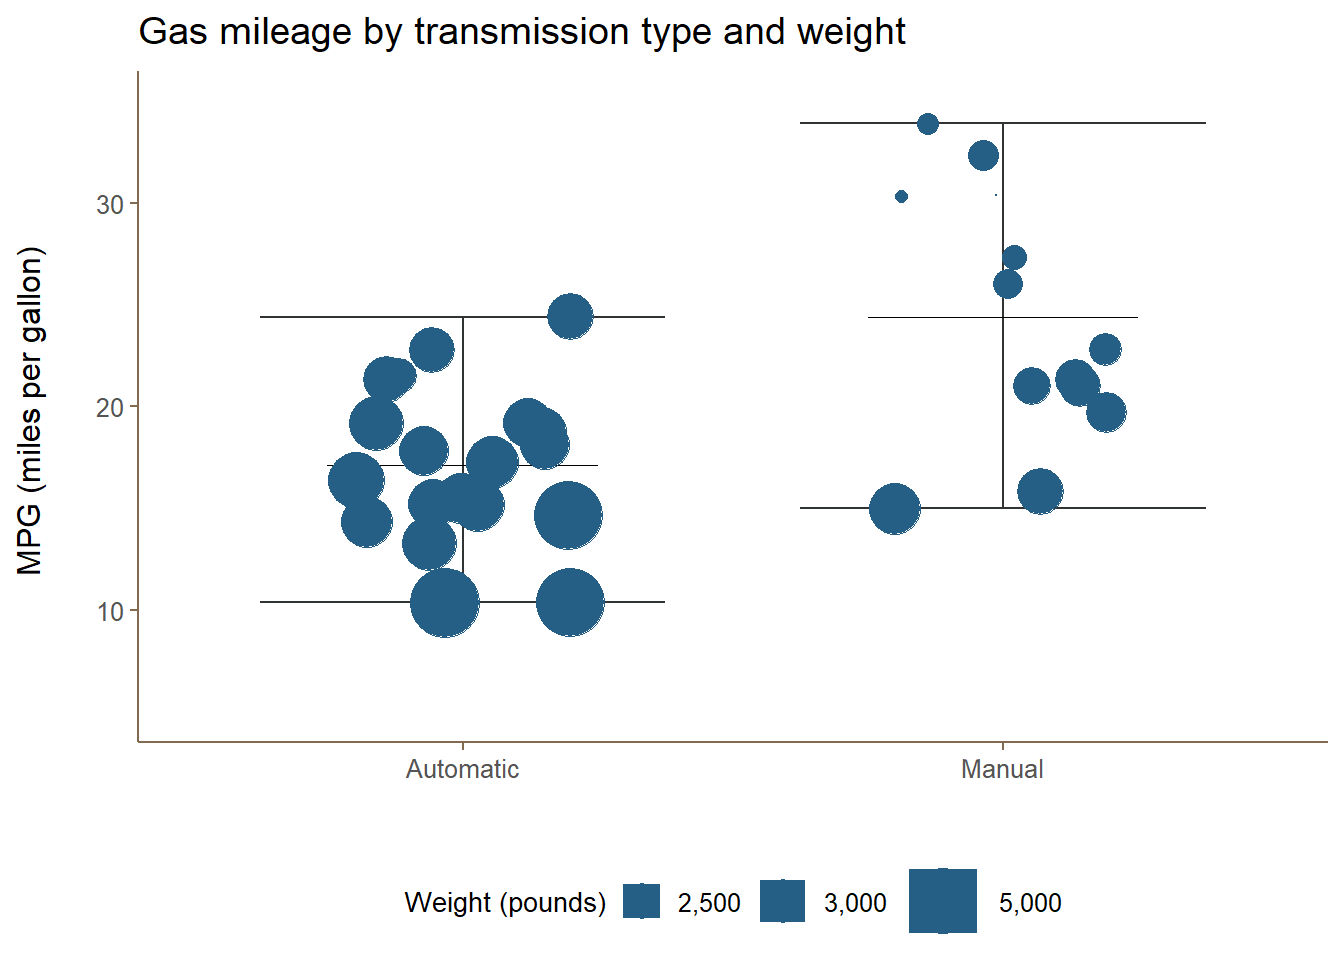
\includegraphics{tooth_analysis_files/figure-latex/unnamed-chunk-3-1.pdf}

\begin{table}[H]

\caption{\label{tab:unnamed-chunk-4}Statistics by Supply Method}
\centering
\begin{tabular}[t]{lrrr}
\toprule
Supply Method & n & mean & sd\\
\midrule
\cellcolor{gray!6}{Ascorbic Acid} & \cellcolor{gray!6}{30} & \cellcolor{gray!6}{16.96333} & \cellcolor{gray!6}{8.266029}\\
Orange Juice & 30 & 20.66333 & 6.605561\\
\bottomrule
\end{tabular}
\end{table}

As a preliminary hypothesis, we can form the first research question
around the supplement type. In general, is expected tooth length larger,
when Vitamin C is supplied as orange juice instead of ascorbic acid?

\begin{verbatim}
## 
##  Welch Two Sample t-test
## 
## data:  len by supp
## t = 1.9153, df = 55.309, p-value = 0.06063
## alternative hypothesis: true difference in means is not equal to 0
## 95 percent confidence interval:
##  -0.1710156  7.5710156
## sample estimates:
## mean in group OJ mean in group VC 
##         20.66333         16.96333
\end{verbatim}

As can be seen, considering 95\% confidence the null hypothesis cannot
be rejected, since the \emph{p}-value is greater than 0.05. So we have
no evidence that there is a significant difference between the two
supplements.

Now, let's see if there is a significant difference between the
supplements at different dosages.

\begin{verbatim}
## 
##  Welch Two Sample t-test
## 
## data:  len by supp
## t = 3.1697, df = 14.969, p-value = 0.006359
## alternative hypothesis: true difference in means is not equal to 0
## 95 percent confidence interval:
##  1.719057 8.780943
## sample estimates:
## mean in group OJ mean in group VC 
##            13.23             7.98
\end{verbatim}

From this result, we see that the data do provide substantial evidence
(\(p < 0.006\)) to reject the null hypothesis \(H_0\), according to
which the expected tooth length is the same when dose of 0.5 mg/day of
Vitamin C is supplied as orange juice.

\begin{verbatim}
## 
##  Welch Two Sample t-test
## 
## data:  len by supp
## t = 4.0328, df = 15.358, p-value = 0.001038
## alternative hypothesis: true difference in means is not equal to 0
## 95 percent confidence interval:
##  2.802148 9.057852
## sample estimates:
## mean in group OJ mean in group VC 
##            22.70            16.77
\end{verbatim}

From this result, we see that the data do provide substantial evidence
(\(p < 0.001\)) to reject the null hypothesis \(H_0\), according to
which the expected tooth length is the same when dose of 1 mg/day of
Vitamin C is supplied as orange juice.

\begin{verbatim}
## 
##  Welch Two Sample t-test
## 
## data:  len by supp
## t = -0.046136, df = 14.04, p-value = 0.9639
## alternative hypothesis: true difference in means is not equal to 0
## 95 percent confidence interval:
##  -3.79807  3.63807
## sample estimates:
## mean in group OJ mean in group VC 
##            26.06            26.14
\end{verbatim}

From this result, we see that the data do \emph{not} provide substantial
evidence (\(p > 0.9638\)) to reject the null hypothesis \(H_0\),
according to which the expected tooth length is the same when dose of 2
mg/day of Vitamin C is supplied either as orange juice or as ascorbic
acid.

\hypertarget{conclusions}{%
\subsubsection{Conclusions}\label{conclusions}}

The data does not provide ample evidence to support the hypothesis that
there is a significant difference between Vitamin C and Asorbic acid
supplements on the expected tooth length of Guinea pigs, However, when
analyzing the dosage level, there is a significant difference for 0.5
and 1 mg. At both the 0.5 mg (\(p < 0.006\)) and 1 mg (\(p < 0.001\))
dosage levels, the data provides evidence to reject null hypothesis in
favor the alternative that expected tooth length is larger when Vitamin
C is provided as the supplement. It is not possible to say that for 2 mg
dose the supplements differ in effects on expected tooth length. The
data do \emph{not} provide substantial evidence (\(p > 0.9638\)) to
reject the null hypothesis \(H_0\), in which the expected tooth length
is the same when dose of 2 mg/day of Vitamin C is supplied as orange
juice.

\end{document}
